\section{Experiments}
\label{sect:experiment}

\FloatBarrier










% \begin{table*}[!ht]
%   \small
%   \caption{Performance of our method combined with SWA and an additional standard teacher. %  on different datasets.
%   }
%   \vspace{0.5ex}
%   \label{table:result-technique}
%   \centering
%   \small
%   \begin{tabular}{clcccccccc}
%     \toprule
%     \multirow{2}{*}{Dataset} & \multirow{2}{*}{Setting} & \multirow{2}{*}{$T$} & \multirow{2}{*}{$\lambda$} & \multicolumn{3}{c}{Robust Acc. (\%)} & \multicolumn{3}{c}{Standard Acc. (\%)}\\
%      & & &  & Best & Last & Diff. & Best & Last & Diff.\\
%     \midrule
%     % \multirow{3}{*}{CIFAR-10} 
%     % & AT & - & - &  $47.35$ & $41.42$ & $ 5.93$ &  $82.67$ &  $84.91$ & -$2.24$ \\
%     % &  KD-AT + KD-Std + SWA & $2$ & $0.5$ & $49.98$ & $49.89$ & $0.09$ & $\textbf{85.06}$ & $\textbf{85.52}$ & -$0.46$\\
%     % & KD-AT-Auto + KD-Std + SWA & $1.47^*$ & $0.8^*$ & $\textbf{50.03}$ & $\textbf{50.05}$ & $\textbf{-0.02}$ & $84.69$ & $84.91$ & $\textbf{-0.22}$\\ 
%     %     \midrule
%     \multirow{3}{*}{SVHN} 
%     & AT & - & - & $47.83$ & $39.77$ & $8.06$ & $90.18$ & $91.11$ & -$0.93$\\
%     & KD-AT + KD-Std + SWA & $2$ & $0.5$ & $47.88$ & $46.46$ & $1.42$ & $\textbf{91.59}$ & $\textbf{91.76}$ & $\textbf{-0.17}$\\
%     & KD-AT-Auto + KD-Std + SWA  & $1.53^*$ & $0.83^*$ & $\textbf{50.58}$ & $\textbf{50.09}$ & $\textbf{0.49}$ & $90.54$ & $90.76$ & -$0.22$\\ 
%     \bottomrule
%     % \tablefootnote{$^*$ indicates the best hyper-parameter searched.}
%   \end{tabular}
% \end{table*}





% \note{Should describe our method again as a whole again? Maybe discuss the difference between our work and Chen et al in more detail in the related work. We further calibrate their method to achieve even smaller overfitting w/o additional human effort.}
% \note{So Why not SWA? Why not clean teacher? Not convenient? Focus on ad training?}
% \chengyu{This section extends to other settings, therefore an independent section}.


% \chengyu{Possible names of methods
% \note{KD-AT}
% \note{AKD-AT (Adaptive knowledge distillation)}
% \note{LabelRectifier}
% \note{Rectified }
% }

% In this section, we verify the effectiveness of our method on multiple datasets. 


\begin{figure*}[t]
  \centering
  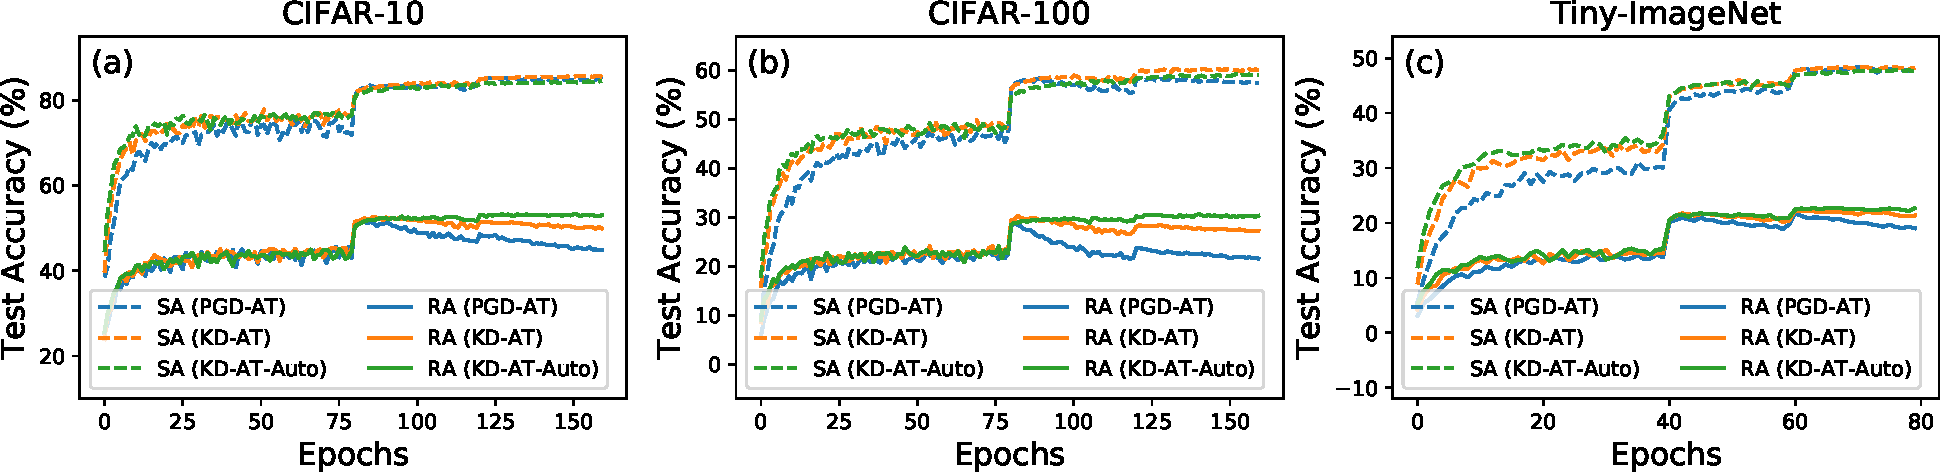
\includegraphics[width=0.98\linewidth]{figures/mitigate-overfitting.pdf}
  \vspace{-1ex}
  \caption{Our method can effectively mitigate robust overfitting for different datasets. 
  }
\label{fig:mitigate-overfitting}
% \vspace{-2ex}
\end{figure*}

% \jingbo{it's a bit odd to me to put the figure in the beginning of a section. }

\smallsection{Experiment setup}
We conduct experiments on three datasets including CIFAR-10, CIFAR-100~\citep{Krizhevsky2009LearningML} and Tiny-ImageNet~\citep{Le2015TinyIV}. We conduct PGD training on pre-activation ResNet-18~\citep{He2016IdentityMI} with $10$ iterations and perturbation radius $8/255$ by default. We evaluate robustness against $\ell_\infty$ norm-bounded adversarial attack with perturbation radius $8/255$, and employ AutoAttack~\citep{Croce2020ReliableEO} for reliable evaluation.  
% We employ SGD as the optimizer with momentum and weight decay set as $0.9$ and $0.0005$ respectively. We conduct the training for $160$ epochs with the learning rate starting at $0.1$ and reduced by a factor of $10$ at epoch $80$ and $120$.
Appendix~\ref{sect:more-result} includes results on additional model architectures (e.g., VGG~\citep{Simonyan2015VeryDC}, WRN),  adversarial training methods (e.g., TRADES~\citep{Zhang2019TheoreticallyPT}, FGSM~\citep{Goodfellow2015ExplainingAH}), and evaluation metrics (e.g., PGD-1000 (PGD attack with $1000$ iterations), Square Attack~\citep{Andriushchenko2020SquareAA}, RayS~\citep{Chen2020RaySAR}). More setup details can be found in Appendix~\ref{sect:exp-setting-all}.

% as an example and include results on TRADES~\citep{Zhang2019TheoreticallyPT} and FGSM~\citep{Goodfellow2015ExplainingAH} in Appendix~\ref{sect:more-result}.  
% The results against more evaluation metrics such as PGD-$1000$ (PGD attack with $1000$ iterations), Square Attack~\citep{Andriushchenko2020SquareAA} and RayS~\citep{Chen2020RaySAR} will be provided in Appendix~\ref{sect:more-result}. 
% We choose pre-activation ResNet-18~\citep{He2016IdentityMI} in the main paper and experiment on more architectures including VGG~\citep{Simonyan2015VeryDC} and WRN in Appendix~\ref{sect:more-result}.



% -------------- Dataset ----------------
\begin{table*}[!t]
  \small
  \caption{Performance of our method on different datasets. $^*$ denotes the hyper-parameters automatically determined by our method. % \chengyu{Results on SVHN. Figure too?}
   }
  \vspace{0.5ex}
  \label{table:result-dataset}
  \centering
  \small
  \begin{tabular}{clcccccccc}
    \toprule
    \multirow{2}{*}{Dataset} & \multirow{2}{*}{Setting} & \multirow{2}{*}{$T$} & \multirow{2}{*}{$\lambda$} & \multicolumn{3}{c}{Robust Acc. (\%)} & \multicolumn{3}{c}{Standard Acc. (\%)}\\
     & & &  & Best & Last & Diff. & Best & Last & Diff.\\
    \midrule
\multirow{3}{*}{CIFAR-10} 
& AT & - & - &  $47.35$ & $41.42$ & $ 5.93$ &  $82.67$ &  $84.91$ & -$2.24$ \\
 & KD-AT & $2$ & $0.5$ &  $48.76$ & $46.33$ & $ 2.43$ &  $82.89$ &  $\textbf{85.49}$ & -$2.60$ \\ 
 & KD-AT-Auto & $1.47^*$ & $0.8^*$ &  $\textbf{49.05}$ & $\textbf{48.80}$ & $ \textbf{0.25}$ &  $\textbf{84.26}$ &  $84.47$ & $\textbf{-0.21}$ \\ 
    \midrule
\multirow{3}{*}{CIFAR-100}
& AT & - & - &  $24.79$ & $19.75$ & $ 5.04$ &  $57.33$ &  $57.42$ & -$0.09$ \\ 
& KD-AT & $2$ & $0.5$ &  $25.77$ & $23.58$ & $ 2.19$ &  $57.24$ &  $\textbf{60.04}$ & -$2.80$ \\ 
& KD-AT-Auto & $1.53^*$ & $0.83^*$ &  $\textbf{26.36}$ & $\textbf{26.24}$ & $\textbf{0.12}$ &  $\textbf{58.80}$ &  $59.05$ & $\textbf{-0.25}$ \\ 
\midrule
\multirow{3}{*}{Tiny-ImageNet} 
& AT & - & - &  $17.20$ & $15.40$ & $ 1.80$ &  $47.72$ &  $47.62$ & $ 0.10$ \\ 
& KD-AT & $2$ & $0.5$ &  $17.86$ & $17.18$ & $ 0.68$ &  $\textbf{47.73}$ &  $\textbf{48.28}$ & -$0.55$ \\ 
& KD-AT-Auto  & $1.23^*$ & $0.85^*$ &  $\textbf{18.29}$ & $\textbf{18.39}$ & $\textbf{-0.10}$ &  $47.46$ &  $47.56$ & $\textbf{-0.10}$ \\ 
    \bottomrule
    % \tablefootnote{$^*$ indicates the best hyper-parameter searched.}
  \end{tabular}
\end{table*}
% \vspace{-1.5em}


\smallsection{Results \& Discussions}
Our method is essentially the baseline adversarial training with a robust-trained self-teacher, equipped with an algorithm automatically deciding the optimal hyper-parameters, which we now denote as KD-AT-Auto.
We compare KD-AT-Auto with two baselines: regular adversarial training (AT), and adversarial training combined with self-distillation (KD-AT) with fixed temperature $T=2$ and interpolation ratio $\lambda=0.5$ as suggested by \citet{chen2021robust}. 

As shown in Figure~\ref{fig:mitigate-overfitting}, our method can effectively mitigate robust overfitting for all datasets, with both standard accuracy (SA) and robust accuracy (RA) constantly increasing throughout training. In Table~\ref{table:result-dataset}, we measure the difference between the RA at the best checkpoint (Best) and at the last checkpoint (Last) to clearly show the overfitting gap. Our method can reduce the overfitting gap to less than $0.5\%$ for all datasets. One may note that self-distillation with fixed hyper-parameters is in fact inferior in terms of reducing robust overfitting, while its effectiveness can be significantly improved with the optimal hyper-parameters automatically determined by our method, which further verifies our understanding of robust overfitting. 
Compared with self-distillation with fixed hyper-parameters, our method can also boost both RA and SA at the best checkpoint for all datasets.


Our method can further be combined with orthogonal techniques such as Stochastic Weight Averaging (SWA)~\citep{Izmailov2018AveragingWL} and additional standard teachers as mentioned in previous work~\citep{chen2021robust} to achieve better performance. More results and discussion can be found in Appendix~\ref{sect:additional-technique}.


% \note{One thing is not doing good is the last standard acc.}


    % We note that employing Equation~(\ref{eq:approximate-label-distribution}) as the supervision in adversarial training with cross-entropy loss is equivalent to the self-training method proposed by~\citet{chen2021robust} without a standard-trained teacher\footnote{We find the standard-trained teacher does not help mitigate the robust overfitting, but rather improve the standard accuracy following a regular knowledge distillation practice.}. 
    % However, the temperature $T$ and the interpolation ratio $\lambda$ have to be manually set in the self-training method, whereas they can be automatically tuned in our method. Figure~\ref{fig:mitigate-overfitting} shows that our automatically-tuned can reduce the overfitting gap better than the fixed hyperparameters for a variety of datasets.
    
    
% \subsection{Combined with additional orthogonal techniques}
% \label{sect:additional-technique}

% Our method can further be combined with other orthogonal techniques such as Stochastic Weight Averaging (SWA)~\citep{Izmailov2018AveragingWL} and additional standard teachers as mentioned in previous work~\citep{chen2021robust} to achieve better performance. 

% More results and discussion can be found in Appendix~\ref{sect:additional-technique}.

% Here, we show that combined with the additional techniques proposed in~\citep{chen2021robust}, our method can achieve better performance.

% We note that our proposed method is essentially the baseline knowledge distillation for adversarial training with a robustly trained self-teacher, equipped with an algorithm that automatically finds its optimal hyperparameters (i.e. the temperature $T$ and the interpolation ratio $\lambda$). Stochastic Weight Averaging (SWA) and additional standard teachers employed in~\citep{chen2021robust} are orthogonal contributions. KD-AT-Auto can certainly be combined with SWA and KD-Std to achieve better performance. 

% We note that the method proposed by \citet{chen2021robust}, namely combining knowledge distillation with self-distillation, an additional standard teacher and SWA (KD-AT + KD-Std + SWA), can already reduce the overfitting gap to almost $0$. It is thus hard to see any further reduction by combining our method. To this end, we introduce an extra dataset SVHN~\citep{Netzer2011ReadingDI}. As shown in Table~\ref{table:result-technique}, on SVHN, the above method KD-AT + KD-Std + SWA still produces a high overfitting gap (also see Appendix A1.3 in~\citep{chen2021robust}), whereas by combining with our method (KD-AT-Auto + KD-Std + SWA), the overfitting gap can be further reduced to almost $0$. This demonstrates the advantage of our principle-guided method on mitigating robust overfitting. More results regarding other datasets and detailed experiment setup can be found in Appendix~\ref{sect:additional-technique}.

% As shown in Table~\ref{table:result-technique}, on CIFAR-10, KD-AT + KD-Std + SWA~\citep{chen2021robust} can already reduce the overfitting gap (difference between the best and last robust accuracy) to almost 0, while KD-AT-Auto + KD-Std + SWA maintains an overfitting gap close to 0. Interestingly, on the SVHN dataset~\citep{Netzer2011ReadingDI}, where KD-AT + KD-Std + SWA still produces a high overfitting gap (also see Appendix A1.3 in~\citep{chen2021robust}), KD-AT-Auto + KD-Std + SWA can further push this gap to close to 0. 

% Here, the interpolation ratio of the standard teacher is fixed as $0.2$ and the SWA starts at the first learning rate decay for all experiments. We employ PGD-AT~\citep{Madry2018TowardsDL} as the base adversarial training method and conduct experiments with a pre-activation ResNet-18. The robust accuracy is evaluated with AutoAttack. Other experiment details are in line with Appendix~\ref{sect: exp-practical}.


% Furthermore, we note that~\citep{chen2021robust} shows SWA and KD-Std are essential components to mitigate robust overfitting on top of KD-AT, while we show that KD-AT itself can mitigate robust overfitting by proper parameter tuning. We are thus able to separate these components and allow a more flexible selection of hyperparameters in diverse training scenarios without fear of overfitting. In particular, although~\citep{chen2021robust} suggests SWA starting at the first learning rate decay (exactly when the overfitting starts) mitigates robust overfitting, the effectiveness of SWA on mitigating overfitting may strongly depend on its hyper-parameter selection including $s_0$, i.e., the starting epoch and $\tau$, i.e., the decay rate\footnote{SWA can be implemented using an exponential moving average $\theta'$ of the model parameters $\theta$ with a decay rate $\tau$, namely $\theta' \leftarrow \tau \cdot \theta' + (1-\tau) \cdot \theta$ at each training step~\citep{Rebuffi2021FixingDA}.}, which is also mentioned in recent work~\citep{Rebuffi2021FixingDA}. We also did some additional experiments on CIFAR-10 following the SWA setting in~\citep{Rebuffi2021FixingDA} to demonstrate the wide applicability of our method. As shown by Table~\ref{table:result-swa}, when changing the hyperparameters of SWA, KD-AT + KD-Std + SWA cannot consistently mitigate robust overfitting, while KD-AT-Auto + KD-Std + SWA can maintain an overfitting gap close to 0 and achieve better robustness as well. 


